\documentclass[25pt, a0paper, landscape, blockverticalspace=-15mm, colspace=15mm]{tikzposter}

\tikzposterlatexaffectionproofoff
\usepackage[utf8]{inputenc}
\usepackage{authblk}
\makeatletter
\renewcommand\maketitle{\AB@maketitle} % revert \maketitle to its old definition
\renewcommand\AB@affilsepx{\quad\protect\Affilfont} % put affiliations into one line
\makeatother
\renewcommand\Affilfont{\Large} % set font for affiliations
\usepackage{amsmath, amsfonts, amssymb}
\usepackage{tikz}
\usepackage{caption}
\usetikzlibrary{matrix}
\usepackage{pgfplots}
% align columns of tikzposter; needs two compilations
\usepackage[colalign]{column_aligned}

\DeclareCaptionFormat{empty}{}
\captionsetup{format=empty}

% tikzposter meta settings
\usetheme{Default}
\usetitlestyle{Default}
\useblockstyle{Default}

%%%%%%%%%%% redefine title matter to include one logo on each side of the title; adjust with \LogoSep
\makeatletter
\newcommand\insertlogoi[2][]{\def\@insertlogoi{\includegraphics[#1]{#2}}}
\newcommand\insertlogoii[2][]{\def\@insertlogoii{\includegraphics[#1]{#2}}}
\newlength\LogoSep
\setlength\LogoSep{-70pt}

\renewcommand\maketitle[1][]{  % #1 keys
    \normalsize
    \setkeys{title}{#1}
    % Title dummy to get title height
    \node[inner sep=\TP@titleinnersep, line width=\TP@titlelinewidth, anchor=north, minimum width=\TP@visibletextwidth-2\TP@titleinnersep]
    (TP@title) at ($(0, 0.5\textheight-\TP@titletotopverticalspace)$) {\parbox{\TP@titlewidth-2\TP@titleinnersep}{\TP@maketitle}};
    \draw let \p1 = ($(TP@title.north)-(TP@title.south)$) in node {
        \setlength{\TP@titleheight}{\y1}
        \setlength{\titleheight}{\y1}
        \global\TP@titleheight=\TP@titleheight
        \global\titleheight=\titleheight
    };

    % Compute title position
    \setlength{\titleposleft}{-0.5\titlewidth}
    \setlength{\titleposright}{\titleposleft+\titlewidth}
    \setlength{\titlepostop}{0.5\textheight-\TP@titletotopverticalspace}
    \setlength{\titleposbottom}{\titlepostop-\titleheight}

    % Title style (background)
    \TP@titlestyle

    % Title node
    \node[inner sep=\TP@titleinnersep, line width=\TP@titlelinewidth, anchor=north, minimum width=\TP@visibletextwidth-2\TP@titleinnersep]
    at (0,0.5\textheight-\TP@titletotopverticalspace)
    (title)
    {\parbox{\TP@titlewidth-2\TP@titleinnersep}{\TP@maketitle}};

    \node[inner sep=0pt,anchor=west] 
    at ([xshift=-\LogoSep]title.west)
    {\@insertlogoi};

    \node[inner sep=0pt,anchor=east] 
    at ([xshift=\LogoSep]title.east)
    {\@insertlogoii};

    % Settings for blocks
    \normalsize
    \setlength{\TP@blocktop}{\titleposbottom-\TP@titletoblockverticalspace}
}
\makeatother
%%%%%%%%%%%%%%%%%%%%%%%%%%%%%%%%%%%%%


% color handling
\definecolor{TumBlue}{cmyk}{1,0.43,0,0}
\colorlet{blocktitlebgcolor}{TumBlue}
\colorlet{backgroundcolor}{white}

% title matter
\title{End to End Learning for Visual Navigation}

\author[1]{Ute Schiehlen}
\author[1]{Natalie Reppekus}
\author[1]{Raymond Chua}

\affil[1]{Technical University of Munich}

\insertlogoi[width=15cm]{tum_logo}
\insertlogoii[width=15cm]{tum_logo}

%adaptions
\definecolorpalette{tumPalette}{
	\definecolor{colorOne}{named}{TumBlue}
	\definecolor{colorTwo}{named}{TumBlue}
	\definecolor{colorThree}{named}{TumBlue}
}
\usecolorpalette{tumPalette}

\usetitlestyle{Empty}
\useblockstyle{Minimal}
\useinnerblockstyle{Minimal}
\colorlet{blocktitlefgcolor}{TumBlue}
\colorlet{innerblocktitlebgcolor}{TumBlue}
\colorlet{notebgcolor}{TumBlue}
\colorlet{notefgcolor}{white}
\colorlet{innerblocktitlefgcolor}{TumBlue}


% main document
\begin{document}

\maketitle

\begin{columns}
    \column{0.4}
    \block{Abstract}{
    An important component in autonomous vehicles is visual navigation. We used a sequence of frames recorded at the front of the car to predict the steering angle using an end to end approach. 
Our network is based on Bojarski et al.\cite{DBLP:journals/corr/BojarskiTDFFGJM16} which consists of five convolutional and three fully connected layers with the steering angle as the training signal. In order to incorporate motion information, we extended this architecture by training an additional convolutional network with {\em optical flow} computed from the images and optimized over the combined loss. As this approach yielded good results, we explored a third architecture consisting of a {\em Long-Short term memory} (LSTM) cell to further exploit temporal information. Our LSTM model achieved an improvement of 0.12 in the Mean Squared Error compared to Nvidia's model.
   }
   
    \block{Data Preprocessing}{
    	\innerblock{Images}{
		\begin{tikzfigure}			
			\hbox{\hspace{-2mm} 
\includegraphics{images/preprocessingImg}}
			%
\includegraphics{images/preprocessingImg}
   		\end{tikzfigure}
	}
	\innerblock{Labels}{
		\begin{tikzfigure}			
			\hbox{\hspace{-2mm} 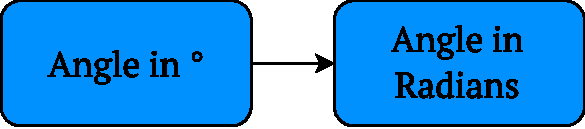
\includegraphics{images/preprocessingLabel}}
			%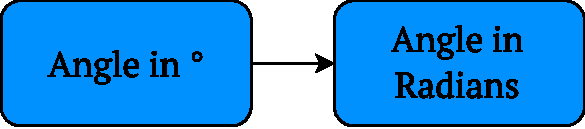
\includegraphics{images/preprocessingLabel}
    		\end{tikzfigure}
	}
    }
    \block{Training and Evaluation Loss}{
    	\begin{tikzfigure}			
		\vbox{\vspace{-10mm} 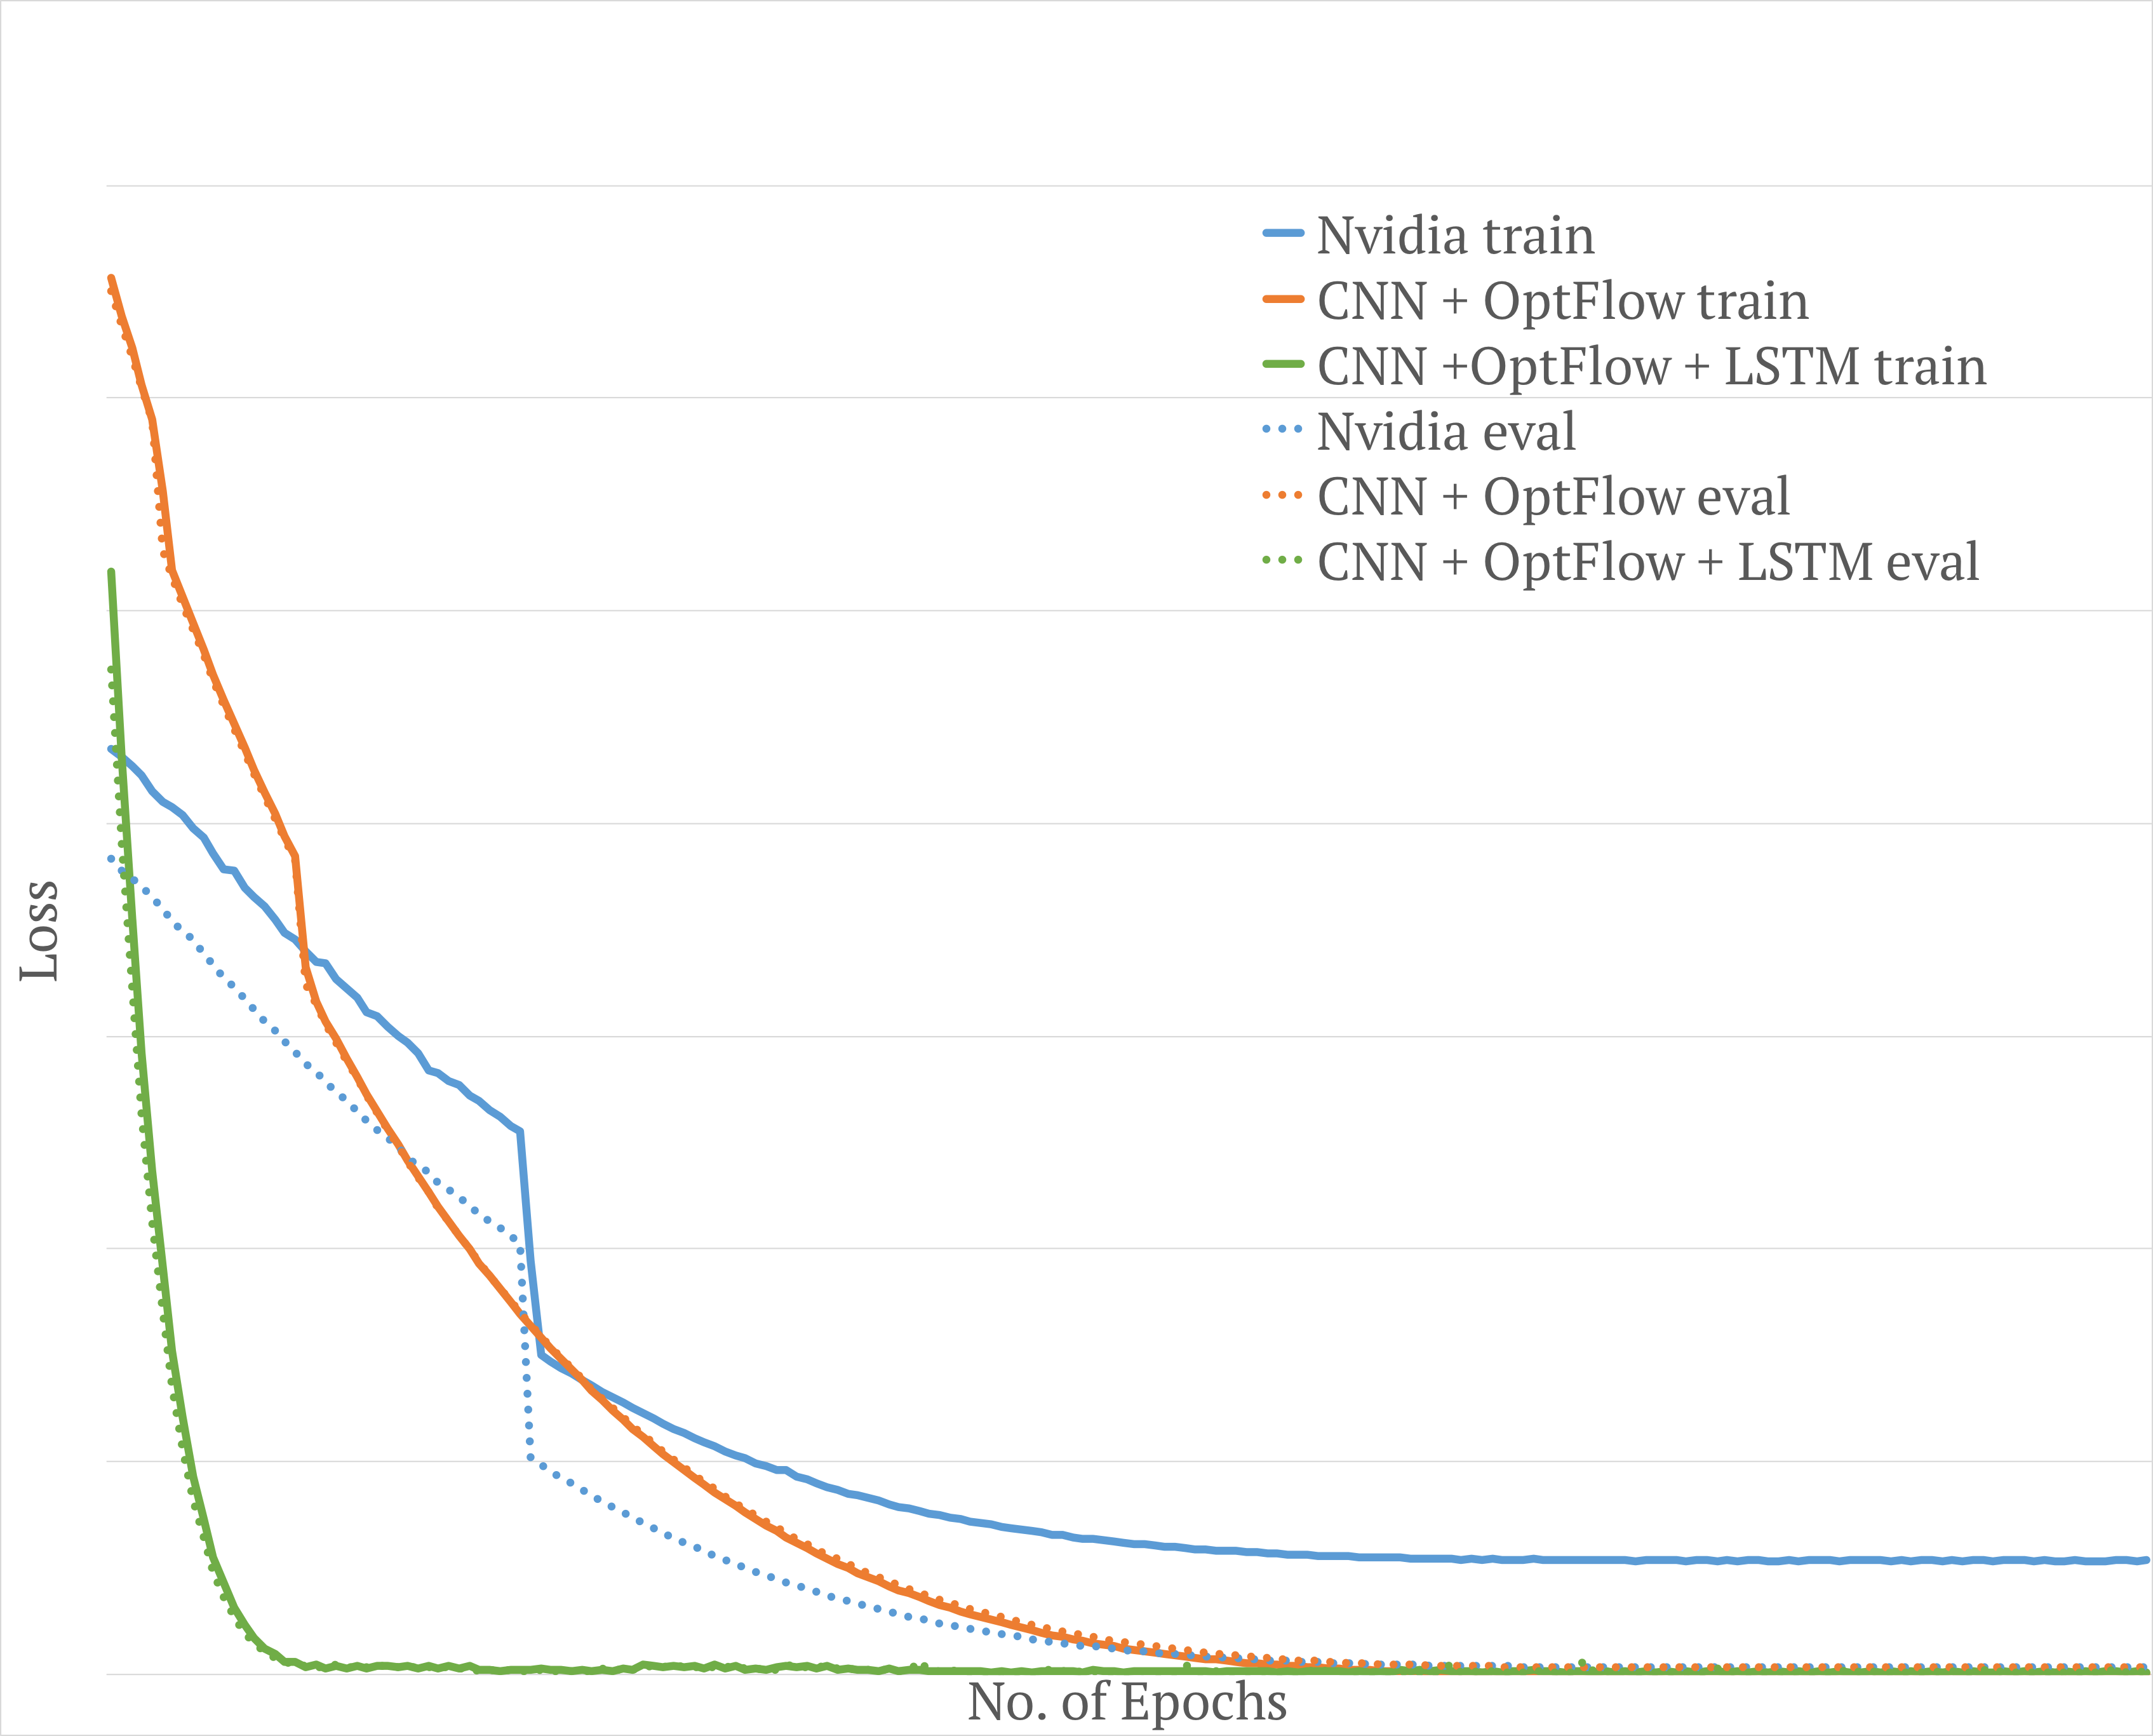
\includegraphics[trim={1 1 1 5cm},clip,scale=0.45]{images/train_eval_v5}}
    	\end{tikzfigure}
    }
    \block{Test Results}{
    	\resizebox{\linewidth}{!}{
	\hspace{-10mm}
	\fontsize{4}{7.2}
	\selectfont
	\begin{tabular}{ c c c c }
		Model & NVIDIA & CNN+OptF & CNN+OptF+LSTM \\
 		\hline
		MSE & 0.1911 & 0.1910  & \textbf{0.072} \\
	\end{tabular}}

	The values above are in radians. Conversion to degrees leads to: $0.19\text{ rad} \approx 11^\circ$, $0.072\text{ rad} \approx 4^\circ$.
    } 
    
    \column{0.2}
    \block{}{
    	\begin{tikzfigure}			
		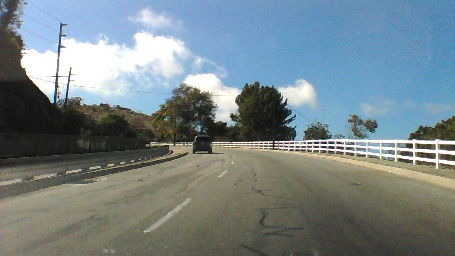
\includegraphics[scale=1.2]{images/img5211}
   	\end{tikzfigure}
	\begin{tikzfigure}			
		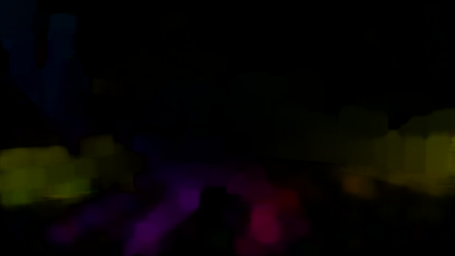
\includegraphics[scale=1.2]{images/opt5211}
   	\end{tikzfigure}
    }
    \block{Loss Functions}{
    	\begin{align*}
	loss_{opt} &= \sum (y_{orig} - labels)^2 + (y_{opt} - labels)^2 \\
	loss_{lstm} &= \sum (y - labels)^2 
	\end{align*}}

    \block{Our Approach}{
    We converted RGB images into YUV color space, which encodes the human perception.We trained all networks using mini-batch Stochastic Gradient Descent with a learning rate of 0.001 over 200 epochs. For the Nvidia and CNN+Optical Flow network, we considered a balanced subset of the training data in order to reduce the number of samples where the car is driving straight. However this was not applied to the LSTM model due to the requirement of having sequential images. In our experiments, we have shown that the LSTM model converges faster during training and achieves a better performance in the testing phase.
     }
    \block{References}{
    	{\footnotesize
		\nocite{*}
		\renewcommand\refname{\vskip -1cm}
		\bibliographystyle{abbrv}
		\bibliography{bib}
	}
    }
    
    \column{0.4}
    \block{Architectures}{
    	\begin{tikzfigure}			
		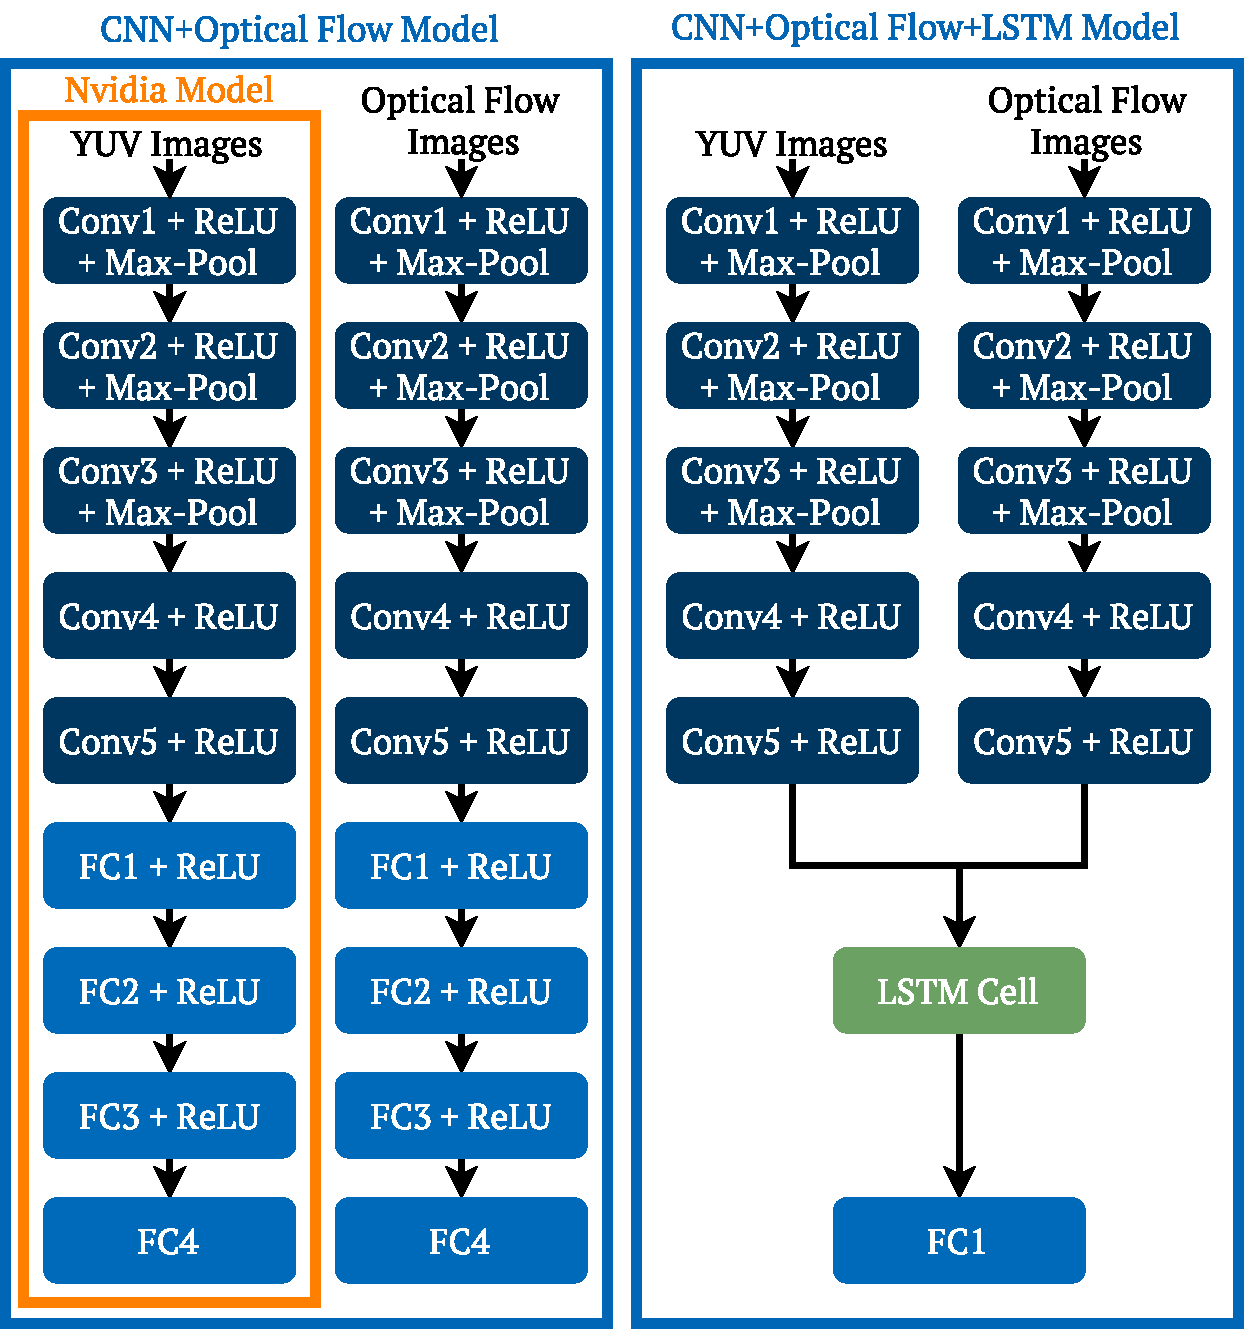
\includegraphics[scale=2]{images/modelOpt}
   	\end{tikzfigure}
	\enspace
	\begin{tikzfigure}			
		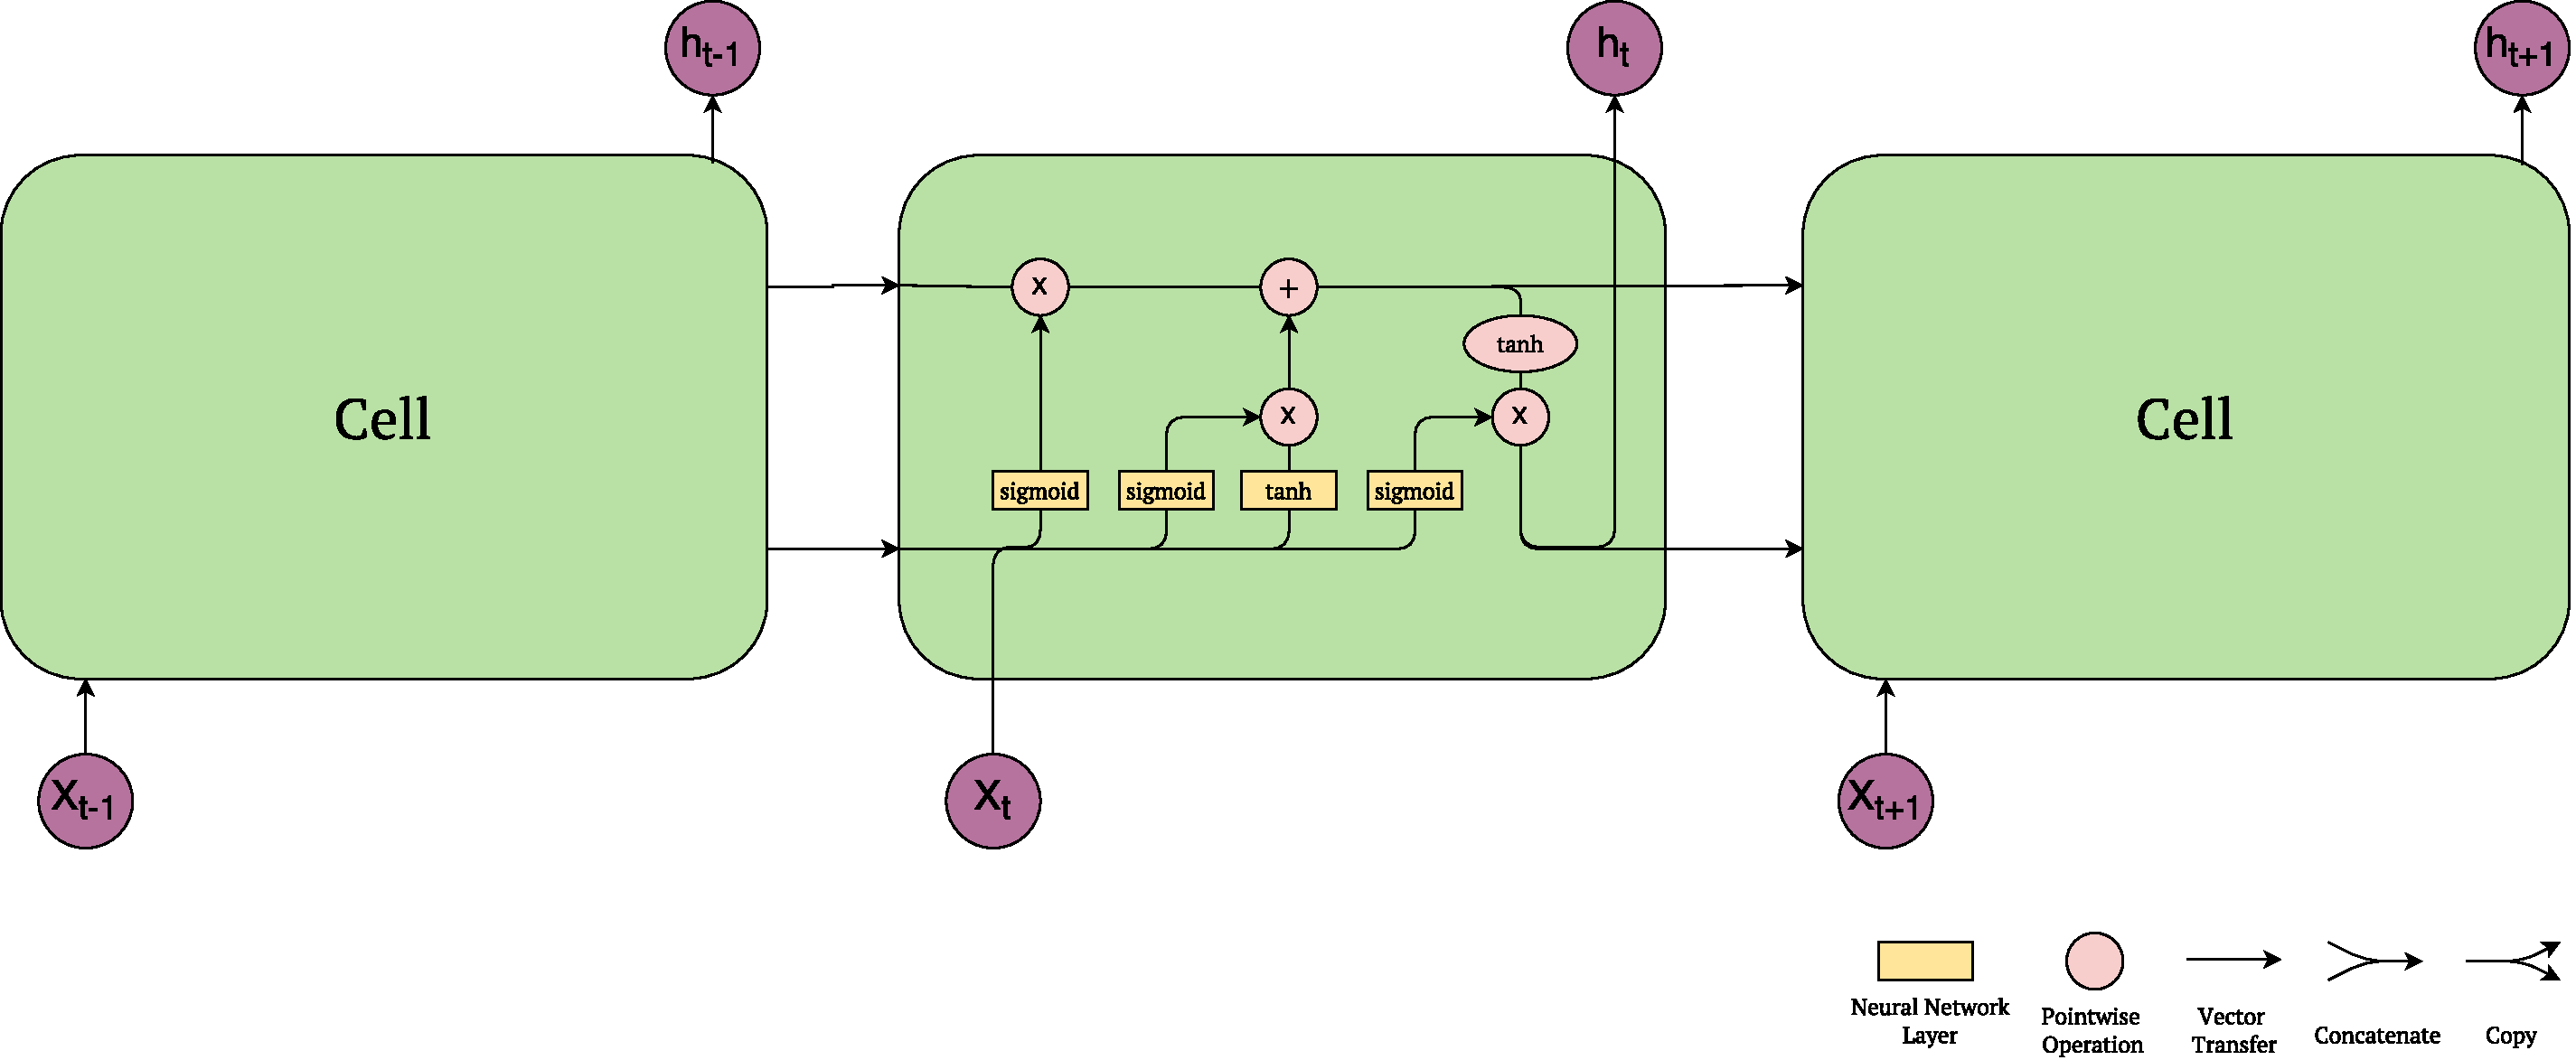
\includegraphics[scale=0.8]{images/LSTM-4}
   	\end{tikzfigure}
    }
    
\end{columns}

\end{document}
